\documentclass{article}
\usepackage{fullpage}

%load needed packages
\usepackage{graphicx}
\usepackage{array}
\usepackage{booktabs}
\usepackage[utf8]{inputenc}
\usepackage[T1]{fontenc}

\usepackage[spanish]{babel} % Paquete para el idioma español
\usepackage{float}  % Necesario para [H]
\usepackage{listings}
\usepackage{xcolor}
\usepackage{url}
\usepackage{tcolorbox}
\usepackage{fancybox} % Paquete para añadir sombras
\usepackage{subcaption}
\definecolor{codegreen}{HTML}{5AB2FF}
\definecolor{morado}{HTML}{AD88C6}
\definecolor{BG}{HTML}{EEEEEE}
\definecolor{azul}{HTML}{4D869C}
\definecolor{sqlblue}{HTML}{FF8C00} % Color para las palabras clave SQL

% Estilo para DDL
\lstdefinestyle{ddlstyle}{
	language=SQL,
	backgroundcolor=\color{BG},
	commentstyle=\color{codegreen},
	basicstyle=\ttfamily\small,
	keywordstyle=\color{azul},
	stringstyle=\color{morado},
	showstringspaces=false,
	breaklines=true,
	frame=shadowbox,
	numbers=left,
	numberstyle=\tiny\color{gray},
	captionpos=b,
}

% Estilo para SQL
\lstdefinestyle{sqlstyle}{
	language=SQL,
	backgroundcolor=\color{BG},
	commentstyle=\color{codegreen},
	basicstyle=\ttfamily\small,
	keywordstyle=\color{sqlblue}, % Color diferente para palabras clave SQL
	stringstyle=\color{morado},
	showstringspaces=false,
	breaklines=true,
	frame=shadowbox,
	numbers=left,
	numberstyle=\tiny\color{gray},
	captionpos=b,
}

\usepackage[utf8]{inputenc}
\usepackage{graphicx}
\usepackage{amsmath}
\usepackage{float}
\usepackage[utf8]{inputenc} % Manejo de caracteres especiales
\usepackage{hyperref}  
\begin{document}




\title{Entrenamiento de CNN para Clasificación de Imágenes COVID-19}
\author{Marta Cuevas Rodríguez}
\date{Diciembre 2024}


	
	% Portada
	\begin{titlepage}
		\centering
		\vspace*{3cm}
		
		% Título destacado
		{\Huge \textbf{Entrenamiento de CNN para Clasificación de Imágenes COVID-19}\\[0.5cm]}
		
		% Espacio y logotipo (si lo tienes, por ejemplo el logo de tu universidad)
		\vspace{2cm}
		
\includegraphics[width=0.3\textwidth]{images/uma_logo.jpg}\\[1cm]
		
		% Nombre del autor
		{\LARGE \textbf{Marta Cuevas Rodríguez}\\[0.5cm]}
		{\large \textit{Herramientas y Algoritmos en Bioinformática}\\
			Universidad de Málaga\\
		}
		
		\vfill
		
		% Fecha en la parte inferior de la página
		{\large Diciembre 2024}
	\end{titlepage}
	
	% Índice
	\tableofcontents
	\newpage
	
	\section{Introducción}
	
	La pandemia de COVID-19, causada por el SARS-CoV-2, desbordó los sistemas de salud a nivel mundial. En la detección y monitoreo de la enfermedad, las radiografías de tórax han jugado un papel fundamental debido a su accesibilidad y rapidez frente a otras pruebas diagnósticas como la RT-PCR. Estas imágenes permiten identificar signos de infecciones respiratorias, como opacidades pulmonares o infiltrados, comunes en COVID-19, neumonía viral y bacteriana, entre otras patologías.
	\\
	
	Este trabajo se enfoca en desarrollar un modelo de red neuronal convolucional (CNN) para clasificar imágenes de radiografías en cuatro categorías: \textit{COVID-19}, \textit{NORMAL}, \textit{PNEUMONIA} y \textit{Lung Opacity}. Para ello, se utiliza el conjunto de datos \textit{COVID-19 Radiography Dataset}, el cual contiene imágenes etiquetadas y balanceadas. El objetivo principal es analizar el rendimiento de las CNN para esta tarea, implementando técnicas de preprocesamiento, aumento de datos y optimización de hiperparámetros.
	
	\section{Objetivos}
	
	El objetivo principal de este proyecto es crear y evaluar un modelo basado en redes neuronales convolucionales (CNN) para la clasificación de imágenes de radiografías de tórax en las categorías \textit{COVID-19}, \textit{NORMAL}, \textit{PNEUMONIA} y \textit{Lung Opacity}.
	
	Los objetivos específicos son:
	\begin{itemize}
		\item Preprocesar y organizar el conjunto de datos \textit{COVID-19 Radiography Dataset} para su uso en el entrenamiento del modelo.
		\item Diseñar y entrenar una red neuronal convolucional (CNN) que clasifique las imágenes en las categorías mencionadas.
		\item Implementar técnicas de aumento de datos para mejorar la capacidad de generalización del modelo.
		\item Ajustar los hiperparámetros y aplicar estrategias como \textit{Early Stopping} para prevenir el sobreajuste.
	\end{itemize}
	
	\section{Configuración Inicial}
	
	El entorno de trabajo fue configurado con las siguientes características:
	
	\begin{itemize}
		\item \textbf{Lenguaje:} Python con TensorFlow \cite{tensorflow2015-whitepaper} y Keras \cite{chollet2015keras}.
		\item \textbf{Hardware:} CUDA para aceleración con GPU (aunque con errores de inicialización).
		\item \textbf{Dataset:} \textit{COVID-19 Radiography Dataset} \cite{rahman2020covid19}., dividido en cuatro clases: COVID, NORMAL, PNEUMONIA y Lung\_Opacity.
		\item \textbf{Preprocesamiento:} Redimensionamiento a $150\times150$ y normalización de imágenes en el rango $[0,1]$.
		\item \textbf{División:} 80\% para entrenamiento y 20\% para validación.
		\item \textbf{Modelo:} Red neuronal convolucional simple.
		
	\end{itemize}
	\newpage
	
	\section{Modelo CNN Simple con Cuatro Clases}
	
	\subsection{Descripción del Modelo}
	
	En este primer enfoque, se implementó una red neuronal convolucional (CNN) simple para clasificar las imágenes en cuatro categorías: \textit{COVID}, \textit{NORMAL}, \textit{PNEUMONIA} y \textit{Lung Opacity}. El modelo consta de:
	\begin{itemize}
		\item Tres bloques de capas \texttt{Conv2D} con activación ReLU y \texttt{MaxPooling2D} para reducir la dimensionalidad.
		\item Una capa densa con 128 neuronas y activación ReLU, seguida de un Dropout del 50\% para evitar el sobreajuste.
		\item Una capa de salida con activación \textit{softmax} para las cuatro clases.
	\end{itemize}
	
	Las imágenes fueron redimensionadas a $150\times150$ com se indicó en la configuración inicial y los valores de los píxeles se normalizaron en el rango $[0,1]$. El modelo fue entrenado con un tamaño de lote inicial de 32, utilizando \textit{categorical crossentropy} como función de pérdida y el optimizador Adam durante \textbf{10 épocas}.
	
	\subsection{Resultados y Análisis}
	
	El modelo alcanzó una precisión global del \textbf{35\%} en el conjunto de validación, con los siguientes resultados por clase:
	
	\begin{itemize}
		\item \textbf{COVID:} Precisión del 17\%.
		\item \textbf{NORMAL:} Precisión del 29\%.
		\item \textbf{PNEUMONIA:} Precisión del 49\%, la mejor entre las clases.
		\item \textbf{Lung Opacity:} Precisión baja del 6\%.
	\end{itemize}
	
Estos resultados indican que el modelo tiene dificultades para distinguir entre las clases, especialmente en la categoría \textit{Lung Opacity}. Las posibles causas de este rendimiento subóptimo incluyen la arquitectura relativamente simple del modelo, que podría no ser suficiente para capturar las características complejas presentes en las imágenes. 
\\

Además, es posible que exista un desbalance en el conjunto de datos, dado que la clase \textit{Lung Opacity} tiene menos muestras que las otras clases, lo que podría dificultar el aprendizaje de patrones representativos para esta categoría. Finalmente, la falta de técnicas de preprocesamiento o aumento de datos más avanzadas podría estar limitando la capacidad del modelo para generalizar mejor en los casos de \textit{Lung Opacity}.
	
	\section{Modelo CNN con Dropout y Early Stopping}
	
	\subsection{Descripción del Modelo}
	
	Para abordar el sobreajuste observado en el modelo anterior, se implementaron dos técnicas de regularización:
	\begin{itemize}
		\item \textbf{Dropout:} Se añadieron capas \texttt{Dropout} del 20\% después de cada bloque convolucional y del 30\% antes de la capa de salida.
		\item \textbf{Early Stopping:} Se configuró un callback para detener el entrenamiento si la pérdida de validación no mejoraba durante 3 épocas consecutivas.
	\end{itemize}
	
	Además, se simplificó el modelo reduciendo la cantidad de neuronas en la capa densa final a 64. El resto de la arquitectura permaneció igual.
	
	Por otro lado, la distribución de los datos en el conjunto de entrenamiento y validación es la siguiente:
	
	\begin{table}[h!]
		\centering
		\begin{tabular}{c c c}
			\hline
			\textbf{Clase} & \textbf{Entrenamiento} & \textbf{Validación} \\
			\hline
			COVID & 5786 imágenes & 1446 imágenes \\
			Lung\_Opacity & 9620 imágenes & 2404 imágenes \\
			Normal & 16308 imágenes & 4076 imágenes \\
			Viral Pneumonia & 2152 imágenes & 538 imágenes \\
			\hline
		\end{tabular}
		\caption{Distribución de las clases en los conjuntos de entrenamiento y validación.}
	\end{table}


	
	
	\subsection{Resultados y Análisis}
	
	El modelo con Dropout y Early Stopping obtuvo una precisión global del \textbf{36\%}, con los siguientes resultados por clase:
	
	\begin{itemize}
		\item \textbf{COVID:} 19\% de precisión.
		\item \textbf{NORMAL:} 28\% de precisión.
		\item \textbf{PNEUMONIA:} 48\% de precisión, la mejor entre las clases.
		\item \textbf{Lung Opacity:} 6\% de precisión.
	\end{itemize}
	
	Los resultados se resumen en la siguiente tabla:
	
\begin{table}[ht]
	\centering
	\caption{Reporte de Clasificación}
	\label{tab:classification_report}
	\begin{tabular}{lcccc}
		\toprule
		\textbf{Clase}       & \textbf{Precisión} & \textbf{Exhaustividad (Recall)} & \textbf{F1-Score} & \textbf{Soporte} \\ 
		\midrule
		COVID                & 0.19               & 0.19                           & 0.19              & 1446             \\ 
		NORMAL               & 0.28               & 0.25                           & 0.26              & 2404             \\ 
		PNEUMONIA            & 0.48               & 0.52                           & 0.50              & 4076             \\ 
		Lung\_Opacity        & 0.06               & 0.05                           & 0.05              & 538              \\ 
		\midrule
		\textbf{Precisión}   &                    &                                 & 0.36              &                  \\ 
		\midrule
		\textbf{Promedio macro} & 0.25               & 0.25                           & 0.25              & 8464             \\ 
		\textbf{Promedio ponderado} & 0.35               & 0.36                           & 0.35              & 8464             \\ 
		\bottomrule
	\end{tabular}
\end{table}
	
	
	
	Durante el entrenamiento, la exactitud de validación superó significativamente la exactitud del entrenamiento (ver Figura \ref{fig:accuracy_curves}). Este comportamiento podría ser causado por sobreajuste, un uso excesivo de la regularización como el Dropout, que pudo haber limitado la capacidad del modelo para aprender patrones complejos, o por la distribución desequilibrada del dataset, que favorece a las clases con más muestras.
	\\
	\begin{figure}[h!]
		\centering
		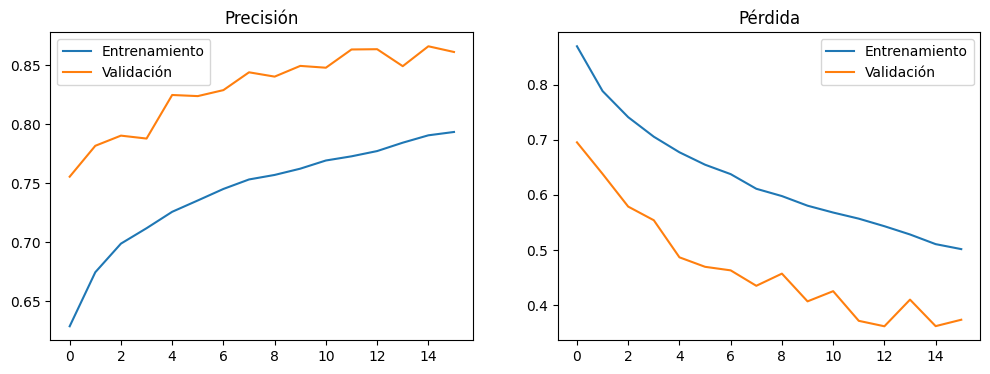
\includegraphics[width=0.8\textwidth]{images/entrenovalidacion1.png}
		\caption{Curvas de exactitud del entrenamiento y validación}
		\label{fig:accuracy_curves}
	\end{figure}

Además, en la curva ROC (Figura \ref{fig:roc1}) se pueden observar que las cuatro clases muestran líneas diagonales, lo que indica que el modelo está realizando predicciones aleatorias. Esto suele suceder debido a un desequilibrio en las clases o un entrenamiento inadecuado, posiblemente por un exceso de regularización. Esto sugiere que el modelo no está logrando diferenciar correctamente entre las clases.

\begin{figure}[h!]
	\centering
	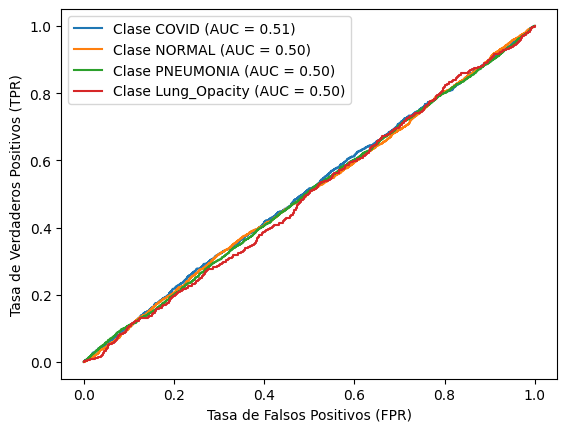
\includegraphics[width=0.8\textwidth]{images/roc1.png}
	\caption{Curva ROC para el segundo modelo}
	\label{fig:roc1}
\end{figure}
	

\newpage

\section{Modificación del modelo y evaluación de desempeño}

En esta etapa, se implementó un modelo basado en una estructura más típica de clasificación de imágenes utilizando una arquitectura de red neuronal convolucional (CNN) con tres capas convolucionales, seguidas de capas de max pooling. Se añadió además una capa densa al final del modelo, junto con una capa de \textit{Dropout} para intentar mitigar el sobreajuste.

\subsection{Cambios implementados}

\begin{itemize}
	\item Se mantuvieron las tres capas convolucionales con un aumento en el número de filtros de 32, 64 y 128 respectivamente, para extraer características más complejas de las imágenes.
	\item Se introdujo una capa de \textit{Dropout} del 50\% después de la capa densa para prevenir el sobreajuste, con la esperanza de que el modelo pudiera generalizar mejor.
	\item Se utilizó la función de activación \textit{relu} para las capas convolucionales y la capa densa, y \textit{softmax} para la salida, adecuada para clasificación multiclase.
	\item La compilación y el entrenamiento del modelo se realizaron utilizando el optimizador \textit{Adam} y la función de pérdida \textit{categorical crossentropy}, ya que es un problema de clasificación multiclase.
\end{itemize}

\subsection{Resultados y Análisis}

Durante las primeras épocas del entrenamiento, los resultados fueron los siguientes: en la primera época, la exactitud de entrenamiento fue de 51.72\%, con una exactitud de validación de 65.90\%. La pérdida en entrenamiento fue de 1.1066, mientras que en validación fue de 0.8270. En la segunda época, la exactitud de entrenamiento aumentó a 63.12\%, y la pérdida en entrenamiento fue de 0.9021.
\\

A pesar de la mejora en la exactitud de validación, la diferencia entre entrenamiento y validación no es suficientemente significativa para considerar que el modelo haya logrado un buen rendimiento generalizado. La exactitud en entrenamiento sigue siendo baja, lo que sugiere que el modelo no ha aprendido de manera efectiva de los datos, indicando un posible subajuste o una arquitectura demasiado simple. Además, la pérdida en entrenamiento es considerablemente mayor que en validación, lo que podría señalar que el modelo no está capturando adecuadamente los patrones en los datos de entrenamiento. Aunque se aplicó una capa de \textit{Dropout} para evitar el sobreajuste, esta no resolvió el problema del subajuste, y el modelo sigue teniendo dificultades para aprender de los datos.
\\

En resumen, a pesar de la implementación de una estructura típica de CNN con \textit{Dropout}, los resultados no muestran mejoras sustanciales. Esto sugiere que el modelo sigue enfrentando problemas tanto en el aprendizaje de las características como en la generalización.



	\section{Análisis del Modelo con MobileNetV2 Preentrenado}
	
	En esta parte, se probó el uso de un modelo preentrenado, específicamente \textit{MobileNetV2}, para mejorar el rendimiento en la tarea de clasificación de radiografías de COVID-19. 
	\\
	
	En esta sección, se utilizó el modelo preentrenado \textbf{\textit{MobileNetV2}} \cite{sandler2018mobilenetv2}, una arquitectura ligera y eficiente diseñada para dispositivos móviles. Este modelo fue preentrenado en el conjunto de datos \textbf{\textit{ImageNet}} \cite{deng2009imagenet}, que contiene millones de imágenes clasificadas en diversas categorías, lo que facilita su adaptación a tareas específicas como la clasificación de radiografías médicas.
	\\ 
	
	A continuación, se detallan las modificaciones realizadas, los resultados obtenidos y un análisis de su desempeño.
	
	\subsection{Modificaciones Realizadas}
	
	Se realizaron las siguientes modificaciones clave:
	
\begin{itemize}
	\item \textbf{Uso de un modelo preentrenado MobileNetV2}: Se cargó MobileNetV2 preentrenado con pesos de ImageNet, excluyendo las capas superiores, para usar solo las capas convolucionales para la extracción de características.
	\item \textbf{Congelación de capas}: Se congelaron las capas de MobileNetV2, excepto por las últimas 50 capas, para que el modelo pudiera seguir aprendiendo sobre características específicas de nuestro conjunto de datos, mientras se aprovechaban las representaciones preentrenadas.
	\item \textbf{Construcción de un nuevo modelo}: Se añadió una capa de \texttt{GlobalAveragePooling2D} después de la base de MobileNetV2, seguida de capas densas con \texttt{ReLU} y \texttt{Dropout(0.5)}, finalizando con una capa \texttt{softmax} para la clasificación multiclase.
\end{itemize}

\subsection{Resultados Obtenidos}

El modelo mostró un rendimiento decente desde el principio, con una precisión de validación del \textbf{74.13\%} en la primera época. Sin embargo, el rendimiento no mejoró significativamente después de esta época. La precisión alcanzada en la validación se estancó y no mostró una mejora sustancial a lo largo de las siguientes épocas.

A pesar de utilizar un modelo preentrenado, el rendimiento no mejoró significativamente en comparación con los intentos anteriores. Esto puede indicar que el \textbf{modelo preentrenado MobileNetV2 no logró ajustarse bien al conjunto de datos}, ya que las características aprendidas de ImageNet pueden no ser lo suficientemente representativas para las radiografías de COVID-19. Además, la \textbf{congelación de capas no fue adecuada}, ya que al congelar muchas de las capas, el modelo no tuvo suficiente flexibilidad para aprender patrones específicos del nuevo conjunto de datos. También, a pesar de contar con un conjunto de datos relativamente grande, la \textbf{cantidad de datos de entrenamiento} podría haber sido insuficiente para que el modelo generalizara correctamente debido a la complejidad del problema. En resumen, aunque el uso de MobileNetV2 preentrenado proporcionó una mejora en el desempeño inicial, no logró un avance significativo con respecto a los modelos anteriores, lo que sugiere que se deben realizar más ajustes y pruebas para mejorar el rendimiento.

	
	\section{Análisis con Modelo Reducido a Dos Clases}
	
	Finalmente, se probó un modelo donde se redujo el número de clases a solo \textbf{COVID} y \textbf{NORMAL}. 
	
	\subsection{Modificaciones Realizadas}
	
	La modificación clave en este experimento fue:
	
	\begin{itemize}
		\item \textbf{Reducción del número de clases}: Se eliminaron las clases \textbf{PNEUMONIA} y \textbf{Lung Opacity}, quedando solo las clases \textbf{COVID} y \textbf{NORMAL} para simplificar el problema y evaluar el rendimiento en un escenario de clasificación binaria.
		\item \textbf{Generación de datos}: Los generadores de datos para entrenamiento y validación fueron configurados para dividir el dataset de manera adecuada, con un 20\% de los datos destinados a validación.
		\item \textbf{Modelo de red neuronal}: Se utilizó una red neuronal convolucional estándar con tres capas convolucionales, capas de max pooling, y una capa densa final con activación softmax.
		\item \textbf{Early stopping}: Se mantuvo la técnica de \textbf{early stopping} para evitar el sobreajuste, monitoreando la precisión de validación y deteniendo el entrenamiento cuando no se observaban mejoras.
		\item \textbf{Prescindir del dropout}: Se decidió prescindir del uso de \textbf{dropout} para permitir que el modelo aprenda mejor las representaciones de los datos sin restricciones adicionales.
	\end{itemize}
	
	
	
	\subsection{Resultados Obtenidos}
	
	El modelo mostró una precisión de \textbf{0.63} en el conjunto de validación. A pesar de que la clase \textbf{NORMAL} presentó un desempeño significativamente mejor, el modelo mostró dificultades para clasificar correctamente las imágenes de la clase \textbf{COVID}.
	
	A continuación se presenta el informe de clasificación obtenido después de entrenar el modelo.
	
	
\begin{table}[ht]
	\centering
	\caption{Informe de Clasificación}
	\label{tab:classification_report}
	\begin{tabular}{lcccc}
		\toprule
		\textbf{Clase}       & \textbf{Precisión} & \textbf{Recall} & \textbf{F1-Score} & \textbf{Soporte} \\ 
		\midrule
		COVID                & 0.27               & 0.23            & 0.25              & 1446             \\ 
		NORMAL               & 0.74               & 0.77            & 0.76              & 4076             \\ 
		\midrule
		\textbf{Precisión}   &  	& &{0.63}                                    &                  \\ 
		\midrule
		\textbf{Promedio macro}   & 0.50               & 0.50            & 0.50              & 5522             \\ 
		\textbf{Promedio ponderado}& 0.62               & 0.63            & 0.62              & 5522             \\ 
		\bottomrule
	\end{tabular}
\end{table}


	
	Aunque los resultados obtenidos aún no son ideales, las curvas de \textbf{accuracy} y \textbf{loss} ( Figura \ref{fig:accuracy_curves2}) muestran un comportamiento más esperado durante el entrenamiento. En la gráfica se puede observar que, a medida que avanzan las épocas, la \textbf{exactitud} en el conjunto de entrenamiento y validación mejora de manera progresiva, lo que indica que el modelo está aprendiendo correctamente de los datos. La \textbf{pérdida}, por su parte, muestra una disminución constante tanto en entrenamiento como en validación, lo cual es una señal positiva de que el modelo está optimizando su capacidad para predecir las clases correctamente. A pesar de que no se alcanzaron los niveles de precisión deseados, las curvas reflejan un rendimiento más estable y coherente en comparación con intentos anteriores, lo que sugiere que el modelo está avanzando hacia una mejor generalización.
	
	
	\begin{figure}[h!]
		\centering
		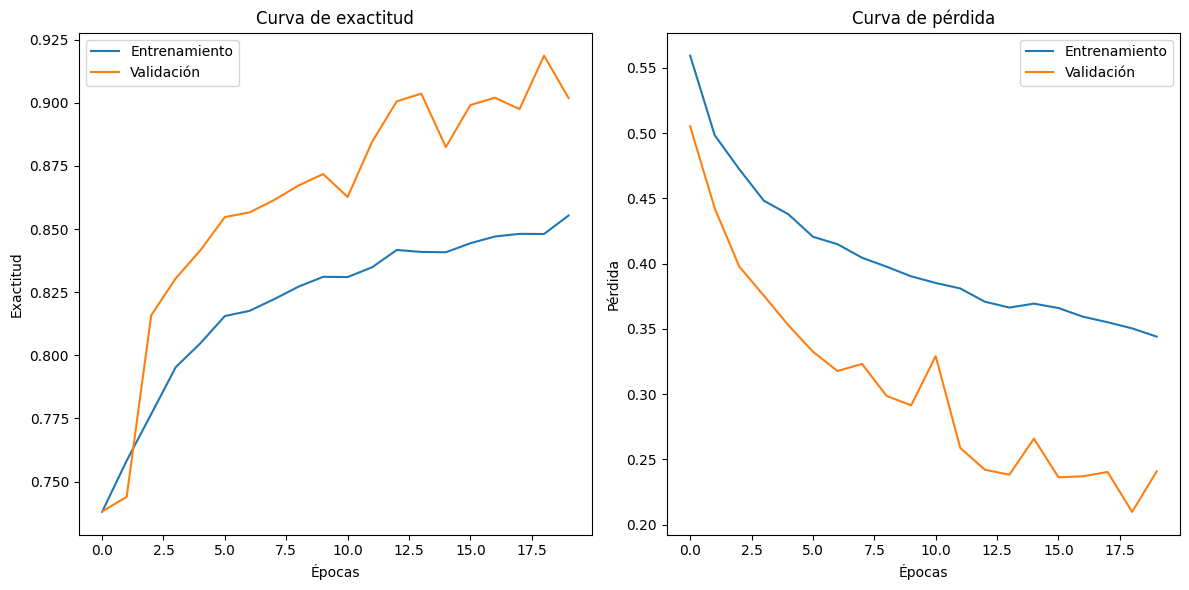
\includegraphics[width=0.8\textwidth]{images/acc-loss.png}
		\caption{Curvas de exactitud del entrenamiento y validación para los conjuntos de datos COVID y NORMAL}
		\label{fig:accuracy_curves2}
	\end{figure}
	
	\begin{figure}[h!]
		\centering
		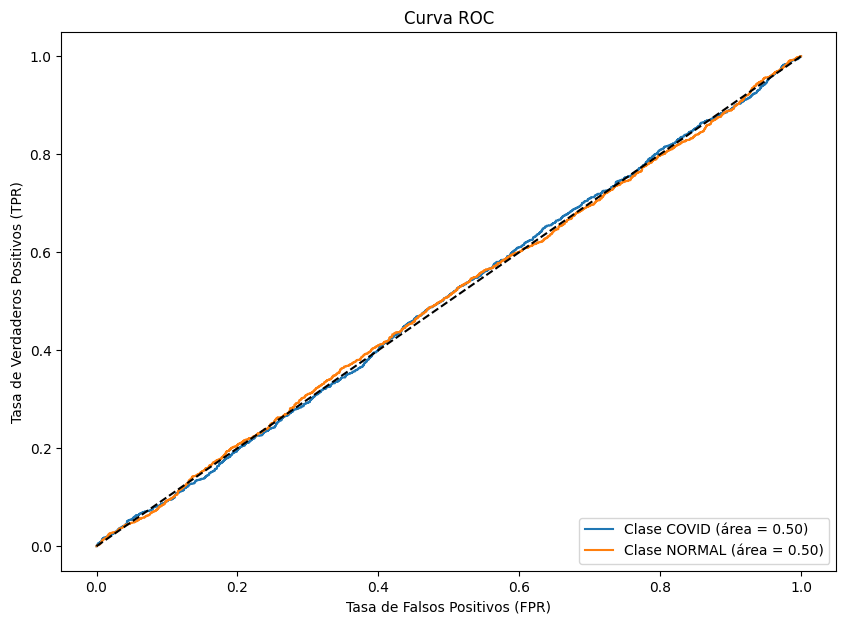
\includegraphics[width=0.8\textwidth]{images/roc2.png}
		\caption{Curvas ROC para los conjuntos de datos COVID y NORMAL}
		\label{fig:roc2}
	\end{figure}

	La curva ROC por su lado (Figura \ref{fig:roc2}), sigue sin mostrar unos resultados coherentes, ya que continúa apareciendo casi diagonal. Esto indica que el modelo no está siendo capaz de distinguir adecuadamente entre las clases, lo que sugiere que el desempeño en la clasificación binaria sigue siendo subóptimo. Una curva ROC diagonal, que representa un modelo aleatorio, indica que el modelo no está aprendiendo patrones útiles de los datos y que la capacidad de discriminación entre las clases sigue siendo insuficiente.
\\

En cuanto a la matriz de confusión, los resultados obtenidos son los siguientes:

	\begin{figure}[h!]
	\centering
	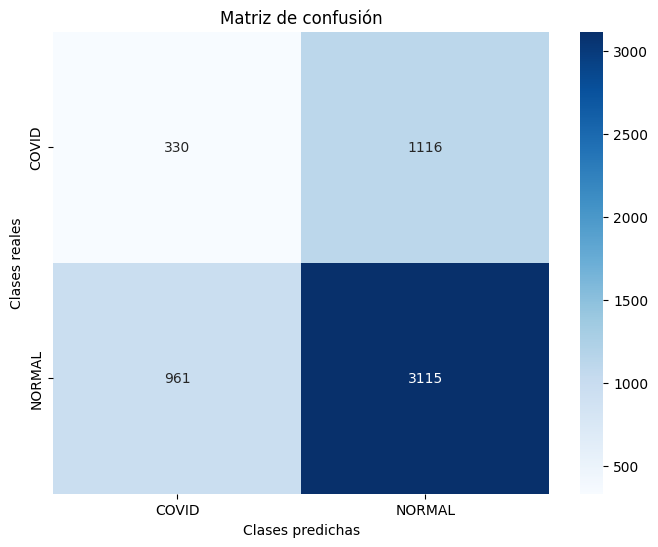
\includegraphics[width=0.8\textwidth]{images/matriz2.png}
	\caption{Matriz de confusión para los conjuntos de datos COVID y NORMAL}
	\label{fig:matriz2}
\end{figure}

Esto indica que, de los 1446 ejemplos de la clase \textit{COVID}, solo 338 fueron correctamente clasificados, mientras que 1108 fueron clasificados erróneamente como \textit{NORMAL}. Por otro lado, de los 4076 ejemplos de la clase \textit{NORMAL}, 3147 fueron correctamente clasificados, mientras que 929 fueron mal clasificados como \textit{COVID}. Esto refleja un claro desajuste en la clasificación de la clase minoritaria \textit{COVID}, lo que está afectando negativamente el rendimiento global del modelo.


\newpage
	
\subsection{Análisis de Resultados}

Durante la experimentación con el modelo reducido a dos clases, se observaron los siguientes puntos clave:

\begin{itemize}
	\item \textbf{Rendimiento desigual entre clases}: La clase \textit{NORMAL} tiene un desempeño significativamente mejor que la clase \textit{COVID}, lo que indica que el modelo podría estar sesgado hacia la clase mayoritaria, \textit{NORMAL}.
	\item \textbf{Desbalance de clases}: Es posible que el conjunto de datos esté desbalanceado entre las clases, lo que podría afectar la capacidad del modelo para aprender características representativas de la clase \textit{COVID}. Se podría explorar el uso de técnicas como el \textit{oversampling} o el \textit{undersampling} para equilibrar las clases.
	\item \textbf{Precisión de validación}: La precisión en el conjunto de validación alcanzó un \textbf{91\%}, lo que sugiere que el modelo tiene un buen desempeño en general, pero podría mejorarse en términos de clasificación de la clase \textit{COVID}.
\end{itemize}

La reducción a dos clases ha mejorado el rendimiento global del modelo en términos de precisión en comparación con el modelo de múltiples clases, pero todavía presenta un desempeño subóptimo para la clasificación de \textit{COVID}.


	\section{Discusión y Conclusiones}
	A pesar de los cambios implementados, el modelo aún presenta un rendimiento subóptimo. Aunque la reducción del problema a dos clases (\textit{COVID} y \textit{NORMAL}) simplificó la clasificación, las dificultades para detectar la clase \textit{COVID} persisten. Las técnicas de aumento de datos y regularización (como el Dropout) contribuyeron a mitigar el sobreajuste, pero no fueron suficientes para mejorar de manera significativa el desempeño del modelo.
	\\
	
	El uso de un modelo preentrenado como MobileNetV2 no proporcionó mejoras sustanciales, lo que sugiere que la naturaleza del conjunto de imágenes, posiblemente con características complejas o difíciles de generalizar, dificulta el entrenamiento. Además, el desbalance de clases entre \textit{COVID} y \textit{NORMAL} probablemente sigue afectando la capacidad del modelo para aprender adecuadamente de la clase minoritaria.
	\\
	
	En resumen, aunque se implementaron varios enfoques para mejorar el rendimiento, el modelo sigue enfrentando desafíos significativos debido a la dificultad del conjunto de datos y el desequilibrio entre clases. Futuras mejoras podrían incluir técnicas más avanzadas de balanceo de clases, métricas adicionales como AUC-ROC para evaluar mejor la clase minoritaria y la implementación de redes más profundas.

\bibliographystyle{plain} % Estilo de bibliografía (puedes cambiarlo)
\bibliography{bibliografia} % Nombre del archivo .bib (sin extensión)


\end{document}

